\documentclass {article}
    \usepackage {graphicx}
    \usepackage[parfill]{parskip}
    \begin {document}
    \title {Automatically Generated Report}
    \author {Elon Musk}
    \date {2020-03-13}
    \maketitle

    \section {Dataset Summary}

    The dataset Births in 1959 has data covering the range of dates between 1959-01-01 and
    1959-12-31. The interval between data points is 1.0 days. Forecasts are calculated
    based on training the model on the 29 days preceding the date being forecasted. The
    mean and median of Births are 41.98 and 42.0
    respectively. Below is the timeseries plot of the data.
    
    \begin {center}
    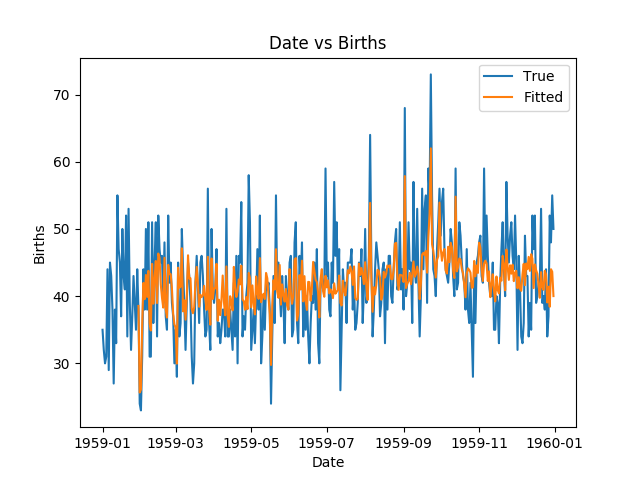
\includegraphics[scale=0.8]{basic_plot.png}
    \end {center}

    \section {Forecast Accuracy}

    The forecast accuracy of the model was evaluated using 2 metrics: mean absolute error (MAE) and root
    mean squared error (RMSE).

    MAE = 4.4

    RMSE = 5.48

    \section {Significant Events}

    The following signficant event dates were captured using a z-score threshold of 3.5:
    
    \begin{center}
     \begin{tabular}{||c c||} 
     \hline
     Date & pctChangeInBirths \\ [0.5ex] 
     \hline\hline 1959-01-13 & 0.67 \\ 1959-01-22 & 0.56 \\ 1959-02-10 & 0.65 \\ 1959-03-03 & 0.61 \\ 1959-03-27 & 0.6 \\ 1959-03-30 & 0.56 \\ 1959-04-11 & 0.56 \\ 1959-09-02 & 0.79 \\ 1959-09-09 & 0.58 \\ 1959-10-28 & 0.57 \\  [1ex] 
     \hline
    \end{tabular}
    \end{center}
    
    The following plot shows the timeseries data along with red dashed lines 
    representing the dates of the significant events.

    \begin {center}
    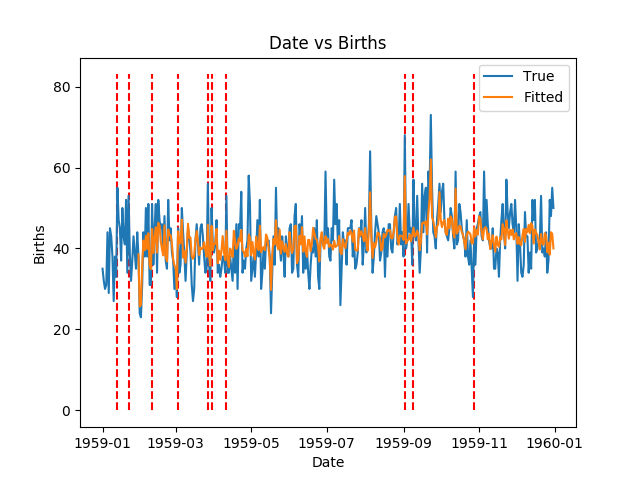
\includegraphics[scale=0.8]{sig_events.png}
    \end {center}

    \end {document}
    